The lead shield and the active vetos were included in the simulation of Tritium-IFIC-2 to quantify the reduction of cosmic background detected. A square plane cosmic ray source of $1~\meter \times 1~\meter$ placed at a height of $70~\cm$ was simulated with the cosmic ray generator of the CRY library. Two R8520-460 PMTs from Hamamatsu were simulated to read out each plastic scintillator, as described in section \ref{sec:IntroductionBackground}. The lead shield was simulated with the lead properties taken from the Geant4 NIST database. The dimensions of the simulated lead shield were $60 \times 60 \times 70~\cm^3$, suitable for one TRITIUM-IFIC-2 prototype and an active cosmic veto but smaller than the real dimension of the lead shield at Arrocampo to optimize simulation time and computing resources. Energy distribution, position and momentum distribution were produced. Simulations with three different shielding configurations were carried out with the aim of quantifying the background rejection due to pasive shield and active veto. The first simulation consisted of one TRITIUM-IFIC-2 prototype and the cosmic ray source. In the second simulation, a lead shield was added and in the third simulation, the cosmic veto was also included. The cosmic events detected by the TRITIUM-IFIC-2 prototype are shown in Figure \ref{fig:CosmicEventsSuppressionSimulated}, according to the shielding configuration. Cosmic rays detected by TRITIUM-IFIC-2 are reduced by a factor around 5.5 when a lead shield $5~\cm$ thick is included (this is the width of the shield currently installed in Arrocampo). This reduction is caused by the suppression of the soft cosmic radiation (energy lower than $200~\MeV$). The natural background of the installation site was not included in this simulation, which is also mitigated by the lead shield, so the expected reduction due to the passive veto would be even better. Around $60\%$ of the cosmic rays that penetrate the lead shield and reach TRITIUM-IFIC-2, which are mostly hard cosmic rays, are detected by the cosmic veto and, therefore, are suppressed from the background. In summary, cosmic rays that would be detected and misidentified as tritium electrons by TRITIUM-IFIC-2 are reduced by a $92.6\%$ by means of the background rejection system and this reduction is expected to be even larger since the natural background of the site was not included in the simulations.

\begin{figure}[h]
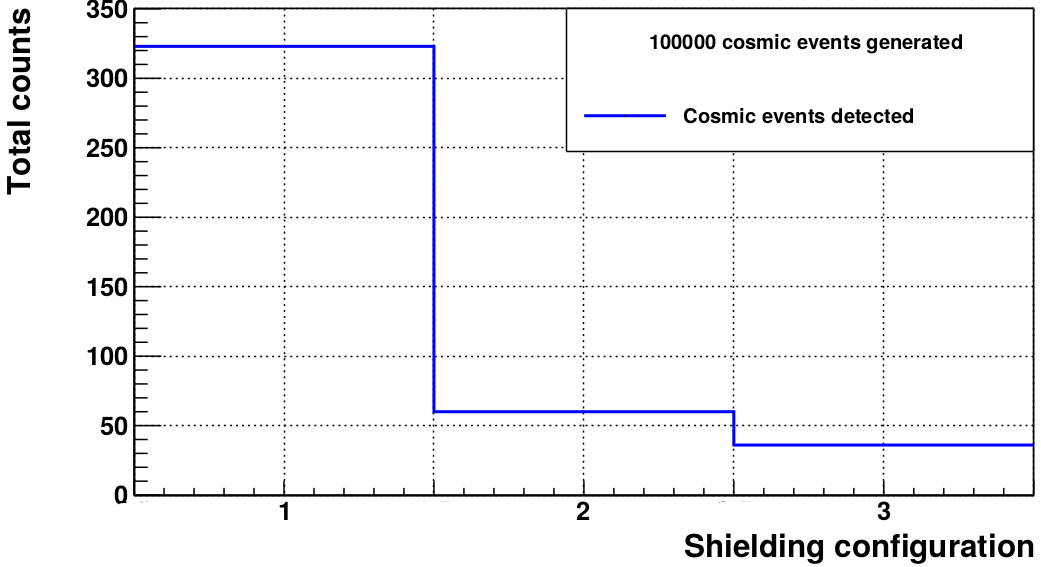
\includegraphics[scale=0.5]{6Simulations/62TRITIUMMonitor/622BackgroundRejectionSystem/Suppression_of_cosmic_events.png}
\centering
\caption{Total cosmic ray events detected by TRITIUM-IFIC-2 from $10^5$ generated cosmic events, which are misidentified as tritium events in three different shielding configurations. Bin 1 corresponds to a no background rejection system. Bin 2 corresponds to the passive shield and bin 3 corresponds to both lead shield and cosmic veto.  \label{fig:CosmicEventsSuppressionSimulated}.}
\end{figure}